% This is samplepaper.tex, a sample chapter demonstrating the
% LLNCS macro package for Springer Computer Science proceedings;
% Version 2.20 of 2017/10/04
%
\documentclass[runningheads]{llncs}
%
\usepackage{graphicx}
\usepackage[portuges]{babel}
\usepackage[T1]{fontenc}
\usepackage{verbatim}
\usepackage{float}
%Path relative to the .tex file containing the \includegraphics command
\graphicspath{ {./images/} }
% Used for displaying a sample figure. If possible, figure files should
% be included in EPS format.
%
% If you use the hyperref package, please uncomment the following line
% to display URLs in blue roman font according to Springer's eBook style:
% \renewcommand\UrlFont{\color{blue}\rmfamily}
\setcounter{secnumdepth}{6}
\renewcommand\theparagraph{\Alph{paragraph}}
 
\makeatletter
\renewcommand\paragraph{\@startsection{paragraph}{4}{\z@}%
                                      {-3.25ex\@plus -1ex \@minus -.2ex}%
                                      {0.0001pt \@plus .2ex}%
                                      {\normalfont\normalsize\bfseries}}
\renewcommand\subparagraph{\@startsection{subparagraph}{5}{\z@}%
                                      {-3.25ex\@plus -1ex \@minus -.2ex}%
                                      {0.0001pt \@plus .2ex}%
                                      {\normalfont\normalsize\bfseries}}
 
\counterwithin{paragraph}{subsubsection}
\counterwithin{subparagraph}{paragraph}
\makeatother

\begin{document}
%
\title{Previsão do estagio de amadurecimento de bananas}
%
\titlerunning{Bananas Maturity Stages Predictions}
% If the paper title is too long for the running head, you can set
% an abbreviated paper title here
%
\author{ Elisa Maia nº \and Henrique Faria nº82200 \and Paulo Barbosa nº }
%
% First names are abbreviated in the running head.
% If there are more than two authors, 'et al.' is used.
%
\institute{Departamento de Informática \and Departamento de Matemática, Universidade do Minho}
%
\maketitle              % typeset the header of the contribution
%
% Abstract
\begin{abstract}

\keywords{}
\end{abstract}
%
%








\newpage
% Introdução
\section{Introdução}
\newpage
\hfill
% Aqui começam os capitulos abordados pelo trabalho
\section{Clusters}

\subsection{Obtenção do número ótimo de clusters}

Para o cálculo do número ótimo de clusters foi utilizada a técnica de \textit{Within Cluster Sum of Squares}. 
Esta algoritmo consiste em escolher k clusters aleatóriamente dos dados que possuimos. Posteriormente calculam-se, para cada ponto, as distâncias Euclidianas entre estes e cada um dos clusters e junta-se cada ponto ao cluster cuja distância é menor.\newline
No fim somam-se as distâncias todas para cada um dos clusters e divide-se pelo número de pontos do cluster obtendo assim a média das distâncias para cada cluster.\newline
Esta técnica foi aplicada para números de clusters que variaram entre 2 e 21. Á medida que o número de clusters aumenta a distância obtida tende para 0, no entanto estamos a tentar identificar o número ótimo de clusters que se pautará pelo melhor compromisso entre divisão em clusters e eficiência. Esta relação é maximizada com a aplicação do método do cotovelo, referido anteriormente, ao gráfico obtido pela representação dos pontos obtidos (cada ponto tem como cordenadas o número de clusters e a distância da soma de quadrados intra-cluster). Aplicando a regra do cotovelo ao gráfico obtido o número de clusters ótimo que obtemos é 6.

\begin{figure}[h]
 
	\centering
 	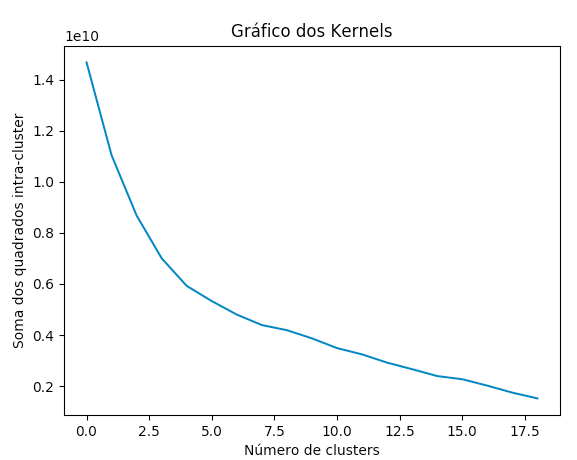
\includegraphics[width=5cm]{kernels_plot.png} 
	\caption{Gráfico da soma de quadrados intra-cluster por número de kernels}
\end{figure}



\subsection{Criação dos clusters com os dados}


Como foi visto anteriormente, os dados estão distribuidos por diferentes canais. Como cada canal tem caraterísticas diferentes não faz sentido criar clusters inter-canais. Por isso vamos criar clusters inter-casos intra-canais.\newline
Para atingirmos este objetivo, começamos por criar um array para cada canal onde reunimos todas as fotografias do nosso dataset de treino pertencentes a esse canal, chamemos D á dimensão deste array. Posteriormente para cada um destes arrays criamos uma matriz de dimensões D x D onde calculamos a distância Euclidiana entre todas as fotografias do array. Note-se que a distância entre uma fotografia e ela mesma é 0, isto leva a que se quisermos juntar os dois clusters mais próximos baseando-nos apenas na distancia independentemente da linha e coluna em que estamos vamos obter sempre uma junção do cluster a si mesmo. Para contornar esta dificuldade em cada linha a distancia do cluster a si mesmo foi substituida pelo dobro da distância máxima entre esse cluster e outro cluster diferente. Adicionalmente foi criado um array de arrays de Labels a que a cada foto existente foi atribuida uma label correspondente ao seu index no array de fotografias. Cada um dos arrays  em que uma label está representa um cluster, assim ao juntarmos clusters podemos juntar igualmente duas labels sem que estas labels sofram alterações numéricas.\newline
Cada matriz que foi criada foi então iterada tantas vezes quanto a diferença entre o número de clusters inicial (no inicio do processo cada foto representa um cluster) e o número ótimo de clusters calculado anteriormente. \newline
A cada iteração um novo cluster foi definido como sendo a junção de dois clusters previanente existentes. Esta junção baseou-se nos dois clusters mais próximos entre si e as distancias calculadas entre este novo cluster e cada um dos restantes clusters são dadas pela distancia média entre cada cluster e os dois clusters anteriores. As labels destes clusters foram também agregadas num mesmo array.\newline
\par Após a agregação das labels representativas das fotografias para cada canal por clusters, temos de atribuir uma mesma label a cada elemento do cluster. Isto é feito recorrendo á label em si que representa a posição da foto no array de fotos, com isto basta-nos percorrer cada array de labels, que corresponde a um cluster e, num segundo array, na posição cujo indice é a label (convêm relembrar que cada label corresponde á posição da fotografia que esta representa no array de fotografias) colocar o número representativo do cluster a que pertence.\newline
Por fim basta-nos reverter a agregação de fotografias por canal e intercalar as labels geradas 11 a 11 entre os arrays representativos dos canais.\newline


\begin{figure}[h]
 
	\centering
 	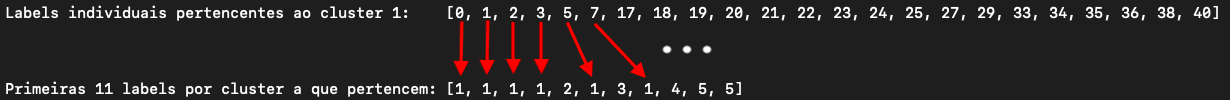
\includegraphics[width=\textwidth]{labelingClusters.png} 
	\caption{Gráfico da soma de quadrados intra-cluster por número de kernels}
\end{figure}





\section{Testes}

Como vimos anteriormente criamos um array de labels que identifica a que cluster pertence cada uma das fotografias que temos. Nesta secção vamos usar tanto essas labels quanto as fotografias para criar uma SVM capaz de classificar fotografias em diversos estágios de maturidade. \newline
Antes de criarmos a SVM devemos ter em atenção alguns problemas que podemos ter com o nosso dataset ou até com as funções usadas na SVM. Para isso iremos numa primeira fase verificar a correção dos casos de treino que possuimos e adicionalmente verificaremos, para cada caso ouconjunto de casos de treino qual a função da SVM que melhor permite destinguir os clusters classificando melhor as fotografias de teste.

\subsection{Preparação}

O primeiro passo a realizar é gerar as combinações de casos de treino a usar no treino da nossa SVM. Para isso foi criado um array que contem as diferentes combinações de casos de treino possíveis (as combinações são independentes da posição em que aparecem os casos).\newline
Adicionalmente foi criado um \textit{switch} que permite alternar entre o tipo das funções usadas para distinguir clusters sendo as opções: \textit{Linear}, \textit{Exponencial} ou \textit{Sigmoid}.

\subsection{Implementação}

Na implementação foi criado um loop para iterar pelas diferentes combinações de casos filtrando todas as fotografias de treino e respetivas labels que não pertencessem aos casos alvo. Em seguida iteramos entre as diferentes hipóteses do \textit{switch} previamente criado para cada conjunto de casos usados de forma a podermos analisar quais as melhores combinações de casos e funções que maximizam a precisão das previsões da nosa SVM.

\subsection{Análise}




%
% ---- Bibliography ----
%
% BibTeX users should specify bibliography style 'splncs04'.
% References will then be sorted and formatted in the correct style.
%
% \bibliographystyle{splncs04}
% \bibliography{mybibliography}
%
\begin{thebibliography}{8}

%\bibitem{ref_intro1}
%https://www.itu.int/en/ITU-D/Statistics/Pages/stat/default.aspx


\end{thebibliography}
\end{document}
